\chapter{Design and Implementation: Porting Xen Split Driver Model to PHIDIAS\label{cha:chapter5}}
For porting Xen split driver model, three major components i.e. Grant tables, Event channels and Xenstore are modified to use static memory and PHIDIAS's xcore and capability feature. In this chapter, I will explain how PHIDIAS's \textit{\textbf{Principle of Staticity}} could be applied to to Xen I/O drivers.

\section{Porting Xen I/O Virtualization Framework to PHIDIAS\label{sec:memstatic}}
All necessary porting done in core components of Xen I/O virtualization framework will be discussed in this section.

\subsection{Porting of Shared Information Pages\label{sec:sharedinfo}}
Shared info page is used to share virtual machine state with Xen hypervisor. It includes information about virtual CPU (vCPU) state, event channels and wall clock time information. Each guest allocates a zeroed page for shared info page from kernel and registers it with Xen hypervisor through a hypercall. In our case, a static memory range has been configured to allocate shared info pages. These pages are shared between guests instead with the PHIDIAS hypervisor. Size of this static memory range is configurable and depends upon the total number of configured guests in system. Each guest obtains its share info page from this static contiguous memory range using its domain ID config option \textbf{CONFIG\_XEN\_DOM\_ID} as shown in listing \ref{sharedpage}. \\
\\
\begin{lstlisting}[caption=Guest mapping its shared information page on PHIDIAS, label={sharedpage}]
Shared_info_pages = (unsigned long)xen_remap(0xfee43000, XEN_PAGE_SIZE * 2);
if (!Shared_info_pages) {
pr_err("not enough memory\n");
return -ENOMEM;
}

if (xen_initial_domain())
memset_io((void *)Shared_info_pages, 0, XEN_PAGE_SIZE * 2);	

HYPERVISOR_shared_info = (struct shared_info *)(Shared_info_pages + (XEN_PAGE_SIZE * CONFIG_XEN_DOM_ID));
\end{lstlisting}
Dom0 with ID 0 initializes the entire range with zeros. The shared info page is mapped in linux guest as un-cached so that other guests would get the consistent view of each other's shared information. Figure \ref{sharedinfo} shows the approach of implementing shared info pages for two guests in PHIDIAS.
\\


\begin{figure}[!htbp]
	\centering
	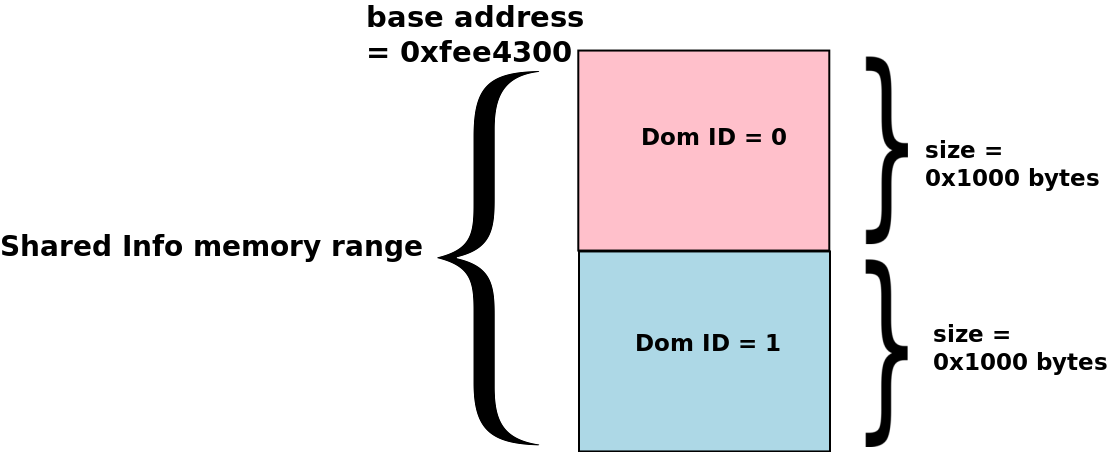
\includegraphics[width=10cm]{sharedinfo}
	\caption{Basic approach of implementation of shared info pages in PHIDIAS for two guests}
	\label{sharedinfo}
\end{figure}


\section{Porting of Grant Tables\label{sec:granttablesstatic}}
As described in \ref{sec:granttables}, grant tables are a mechanism for sharing memory pages across domains. Xen hypervisor allocates pages for grant tables per domain and guests map them into their address spaces. By design, Xen does not support swapping which means that even unused part from the allocated memory of a guest could not be used by other guests. To solve this problem, Xen uses \textbf{ballooning}. Ballooning is way of dynamically increasing or decreasing size of allocated memory. Memory visible to each guest can be configured in Xen at boot time. For Dom0, it could be specified in grub configuration file and for domU, it is specified in XL tool's guest configuration file. If the guest uses less memory than configured amount, it can return unused blocks of memory to hypervisor. However, guest can not retrieve more memory from hypervisor's memory pool through ballooning than its maximum configured amount specified during its startup. Memory allocated to unprivileged guests is taken from Dom0 memory pool and hence Dom0 memory balloon's down every time a new guest is started.
\\
\\
For the current work, Xen balloon driver has been disabled in Linux guest kernel using configuration option CONFIG\_XEN\_BALLOON. In the native code of Xen's PV split drivers, ballooning is used to allocate pages for grant tables, XenBus ring buffers and mapping received network packets in network backend driver from the related frontend. In our ported setup, it has been replaced by defining two static globally shared readable/writable memory ranges for PHIDIAS's guests. One memory range is defined to allocate static memory for grant table frames while the other is defined to be used by all split drivers for establishing communication for I/O virtualization. Guests allocates required pages from these two memory ranges and map them un-cached into their respective address spaces. These two memory ranges will be explained in more detail in the following sections.

\subsection{Static Memory for Grant Frames\label{sec:granttablesframes}}
In Xen, maximum number of grant frames is defined to be 32. For the current thesis, since two guests were used for testing, a total of 64 contiguous pages had been configured for grant tables usage. Each guest had used 32 pages for its own grant table implementation. In our setup, every guest had access to other guests' grant table through un-cached mapping of their grant pages into its address space. For performing grant table operations, I/O split drivers of Xen find a reference or index of unused entry in their guest's grant tables and update this entry with fields of corresponding domain ID, shared frame number and desired flags. The guest then sends the obtained grant reference through ring buffers to the other guest. In native Xen setup, hypercalls are used to perform grant operations i.e. granting access to remote domain, mapping, transferring and copying pages across domains. In our ported setup, since each guest had access to remote's dguest's grant tables by mapping them directly into its address space, a local guest could perform direct operations by manipulating the fields in grant table entries of a remote guest. Listing \ref{grantmap} shows how a guest mapped remote guest's grant table into its domain in our setup. Figure \ref{grant_table} shows the configuration of grant table static memory range for two guests in PHIDIAS.
\begin{figure}[!htbp]
	\centering
	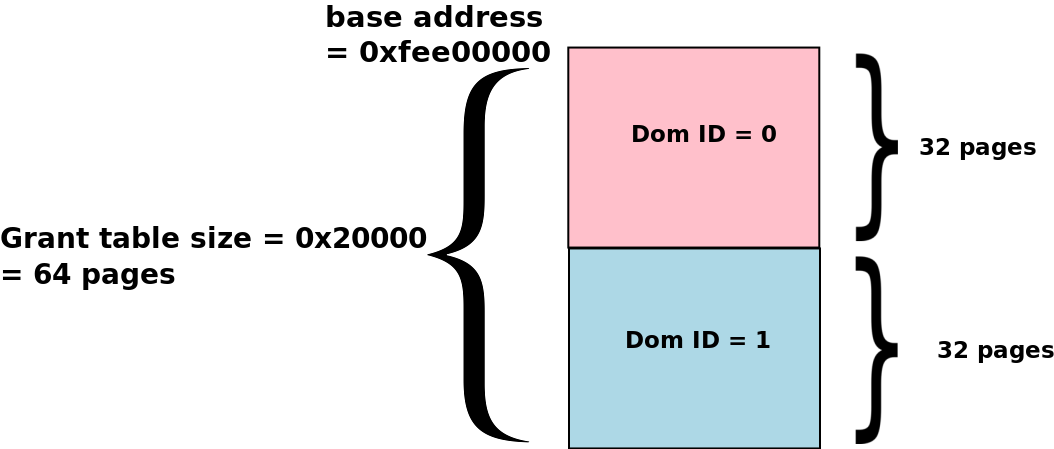
\includegraphics[width=10cm]{grant_table}
	\caption{Static memory configuration for grant table in PHIDIAS for two guests}
	\label{grant_table}
\end{figure}
\begin{lstlisting}[caption=Code snippet for mapping remote guest's grant table in case of two guests configured for the ported setup , label={grantmap}]
static int gnttab_setup(void)
{ ...
        gnttab_shared.addr = xen_auto_xlat_grant_frames.vaddr;
        
        if(xen_initial_domain())
            remote_grant_frames = 0xfee00000 + (0x20000 * 1) ;
        else
            remote_grant_frames = 0xfee00000 + (0x20000 * 0) ;
            
        vaddr = xen_remap(remote_grant_frames, XEN_PAGE_SIZE * max_nr_gframes);
        
        gnttab_shared_remote.addr = vaddr;
...
}
\end{lstlisting}

\subsection{Static Memory for I/O Split Drivers Usage\label{sec:splitdriverusage}}
I/O Split drivers of Xen guests play with memory using a set of in-built kernel functions e.g alloc\_page, free\_page etc. However, they share those pages with other guests through Xen's grant table hypercalls. In order to use the same Linux page allocation APIs and keep changes in split drivers as minimum as possible, a new memory zone named \textbf{ZONE\_XEN} had been added in Linux kernel for our setup. A static globally- shared memory range of size 8192 KB has been configured in PHIDIAS for two guests. Size of ZONE\_XEN for each guest was set to 4096 KB i.e. 1024 pages. Each guest obtained the starting address of its zone using the base address of configured shared memory range of size 8192 KB and its domain ID as shown in listing  \ref{list_zone}.
\\
\begin{lstlisting}[caption=Code snippet for calculating start address of guest ZONE\_XEN, label={list_zone}]
    xen_zone_size = 0x400000;
    xen_zone_start_addr = 0xfef00000 + (CONFIG_XEN_DOM_ID * xen_zone_size);

\end{lstlisting}
Figure \ref{zone_xen} shows the memory configuration for areas of ZONE\_XEN for two guests in PHIDIAS.
\begin{figure}[!htbp]
	\centering
	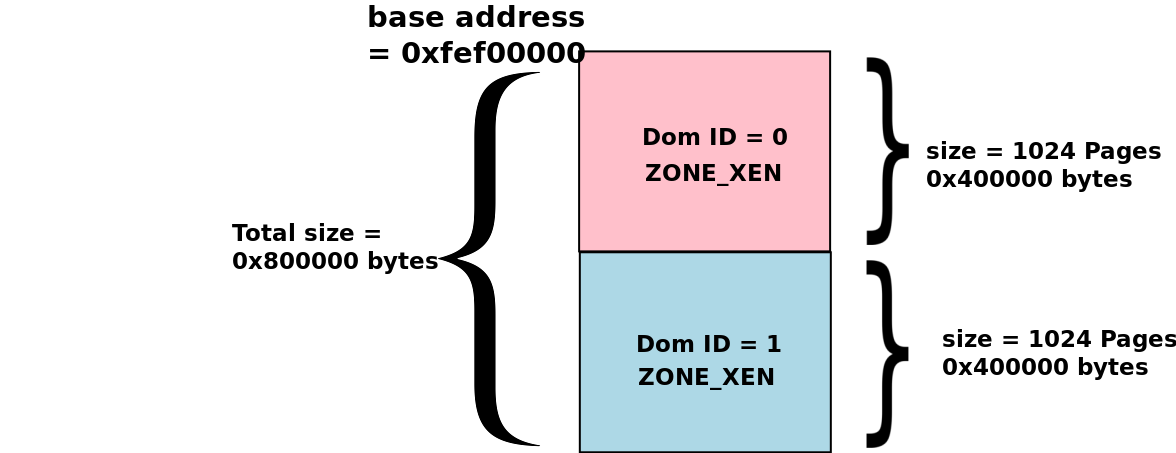
\includegraphics[width=10cm]{zone_xen}
	\caption{Static memory configuration for ZONE\_XEN in PHIDIAS for two guests}
	\label{zone_xen}
\end{figure}
Since the entire zone memory range is shared between two guests in our setup, each guest could easily calculate the starting address of other guest's zone space. In order to access pages granted for sharing by a remote's guest, the local guest should map those pages into its address space so that it could read or write on those shared pages. In native Xen setup, Xen hypervisor is responsible for modifying page tables and sharing of pages across domains. However, in our setup, we have to map all pages of other's guest ZONE\_XEN into local guest address space before accessing them through I/O split drivers. We cannot use \textbf{ioremap} function when grant operations are called by split I/O driver e.g in \_\_gnttab\_map\_grant\_ref and gnttab\_batch\_copy. The reason is that ioremap cannot be called in interrupt context and PV split drivers perform grant operations in this particular context. In order to solve this problem, whole zone area of other guest had been mapped in local guest's address space during initialization in arch\_gnttab\_init function as shown in listing \ref{hash}.\\
\\
\begin{lstlisting}[caption=Code snippet for populating hash table for virtual address mapping of shared pages for two guests in ported setup, label={hash}]
int arch_gnttab_init(unsigned long nr_shared)
{ ...

#if CONFIG_XEN_DOM_ID == 1
base_value = 1044224;
phys_addr = 0xfef00000;

#elif CONFIG_XEN_DOM_ID == 0
base_value = 1045248;
phys_addr = 0xFF300000;
#endif


virt_addr =  xen_remap( phys_addr , 0x400000);
for (i = 0; i< SIZE_ARRAY; i++)
{
key = phys_addr >> XEN_PAGE_SHIFT; 
hash_insert(key, virt_addr);
virt_addr = (unsigned long)(virt_addr) + 4096;
phys_addr = phys_addr + 4096;
}
..
}
\end{lstlisting}
Then a hash table had been created containing virtual addresses of these mapped pages indexed with their respective physical page frame numbers. This hash table had thus solved the following two problems:

\begin{itemize}
	\item Speed up the process of finding virtual address of remote's guest shared page by not mapping each page individually in grant table functions.
	\item Avoiding the use of ioremap in grant table functions since it cannot be called in interrupt context.
\end{itemize}

Figure \ref{hash_table} shows the basic structure of implemented hash table.

\begin{figure}[!htbp]
	\centering
	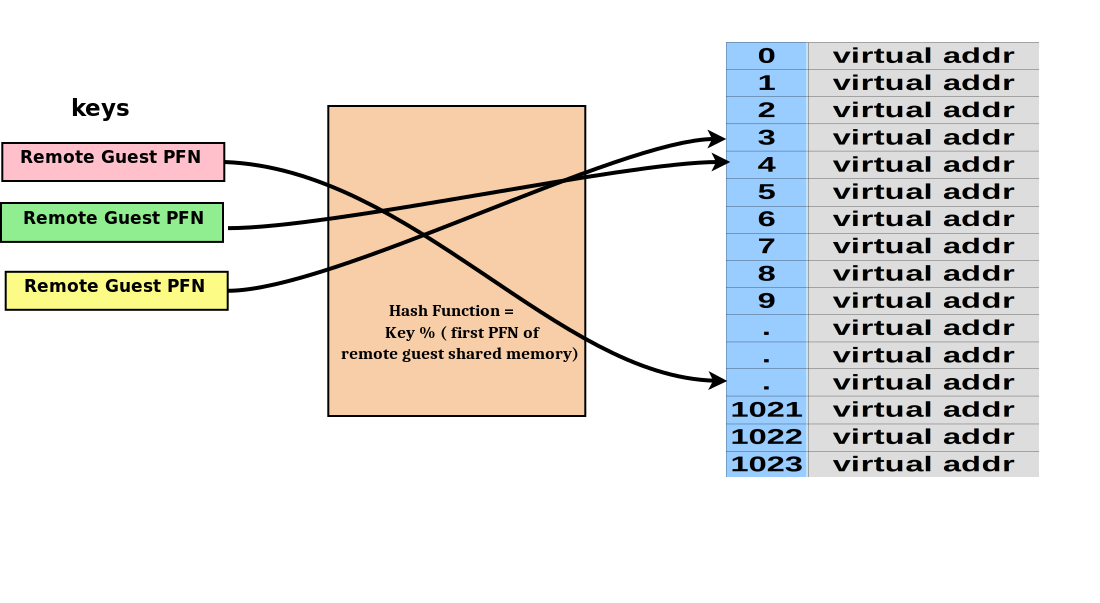
\includegraphics[width=10cm]{hash_table}
	\caption{Structure of hash table used for accessing remote guest's of ZONE\_XEN shared pages}
	\label{hash_table}
\end{figure}


\section{Design of Porting Event Channels\label{sec:eventstatic}}
As explained in section \ref{sec:eventchannel}, event channels are used to send asynchronous notifications among guests in Xen. On ARM, software generate interrupts (SGI) can be used for interprocessor communication. There are 16 SGI available on ARM architecture. For Xen guests, there is a common interrupt handler \textbf{xen\_arm\_callback} for handling notifications from remote guests via event channels. Xen guest uses PPI 31 for event IRQ which is configured in hypervisor node of its flattened device tree provided to it by Xen during its booting sequence as shown in listing \ref{xen_node}.
\\
\\
\begin{lstlisting}[caption=Xen Hypervisor node in hi6220 flattened device tree, label={xen_node}]
 hypervisor {
     compatible = "xen,xen", "xen,xen-4.7"; //version of the Xen ABI 
     reg = <0xb0000000 0x20000>;            // Grant table memory area 
     interrupts = <1 15 0xf08>;             //event notifications IRQ
 };

\end{lstlisting}
In PHIDIAS, SGIs have been used for implementing interprocessor interrupts using its \textbf{Xcore mechanism}. By default, first 6 SGI interrupts are used by Linux kernel. In our ported setup, we could use one of the remaining SGIs for registering \textbf{xen\_arm\_callback} handler for Xen event IRQ. However, in Linux kernel version 4.11\_rc2 used in this work, Linux kernel handle\_IPI function only processes first 6 SGIs. For remaining SGIs, it shows a default warning of \textit{Unknown IP}. To handle this, some modifications were made in IPI handling code of Linux kernel. For SGIs other than the default first six, modified IPI handling function is implemented for our setup. It checked whether some handler is registered for given interrupt number and then called respective handler if found any. An online resource \cite{smp} has been used as a reference for implementing this IPI handling function.
\\
\\
I had used SGI number 9 for triggering Xen events in PHIDIAS for inter-domain communication. 2-level event channel support had been ported which used two-level bitmap to speed searching. The first level is a bitset of words which contain pending event bits.  The second level is a bitset of pending events themselves. All event channel hypercalls in Xen guests were replaced with PHIDIAS specific code working on shared memory and Xcore capabilities. 

\subsection{Static Memory Allocation for Event Domain Pages \label{sec:eventsdomains}}
Xen hypervisor maintains a structure for event channels per domain which stores necessary information e.g. VCPU for local delivery notification, event channel type, port number and priority etc. When a guest issues hypercall to send an event to a remote guest, Xen hypervisor uses this structure to find remote domain ID and remote port and injects interrupt into destination guest. 
\\
\\
In current work, all maintenance of event domain structures and triggering of IPI had been moved into guest domain. For remote sharing of Xen event domain structures, a static globally shared memory named \textbf{event\_domains} has been configured in PHIDIAS and mapped into guests' domains. In our implementation, the number of event channels each guest could support was limited to the amount of event domain structures that a single page could hold. Each guest had access to remote guest's event domain page containing an array of event domain structures so that it could write its domain ID and local event port number while binding inter-domain event channels. Figure \ref{event_domains} shows the basic structure of event domains pages in PHIDIAS for two guests.

\begin{figure}[!htbp]
	\centering
	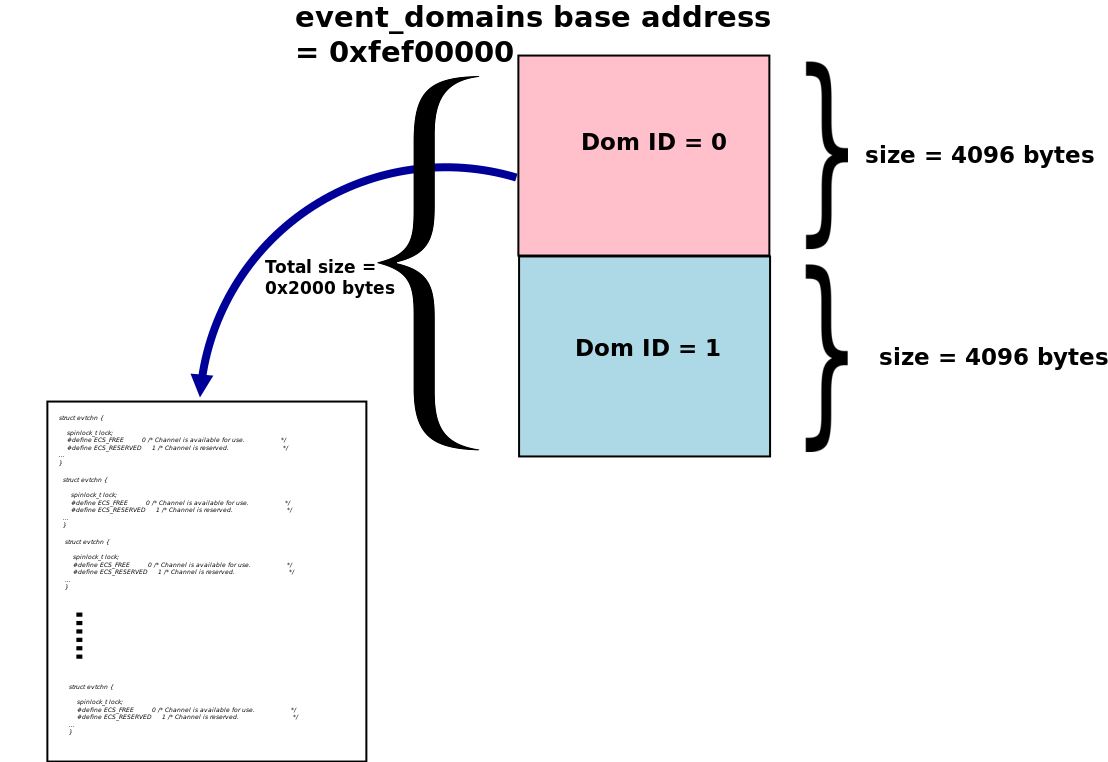
\includegraphics[width=10cm]{event_domains}
	\caption{Basic structure of shared event domains pages in PHIDIAS for two guests}
	\label{event_domains}
\end{figure}

\subsection{Adding Capabilities for IPI in PHIDIAS \label{sec:eventsdomains}}
In Xen split driver model, virtual guests use event channels in two scenarios:
\begin{itemize}
	\item Sending event notifications between Xenstore userspace application and PV I/O drivers, behaving more like an intra-domain event.
	\item Sending event notifications between frontend and backend of split drivers, behaving more like an inter-domain event.
\end{itemize}
For the above two types of events, two capabilities had been added in guest configuration on PHIDIAS as shown in listing \ref{cap}.\\

\begin{lstlisting}[caption=Capabilities added for event notifications in guest configuration on PHIDIAS, label={cap}]
For Dom0 Linux guest 1
      <cap type="ipc" target_xref="linux2" param="0x9" /> 
      <cap type="ipc" target_xref="linux1" param="0x9" /> 
For DomU Linux guest 2
      <cap type="ipc" target_xref="linux1" param="0x9" /> 
      <cap type="ipc" target_xref="linux2" param="0x9" /> 
\end{lstlisting}

Both capabilities had type \textbf{ipc}. First capability had index 0 with destination selected to be remote guest and second capability had index 1 with destination chosen to be itself. First capability was used for \textbf{inter-domain events} and second capability emulated \textbf{intra-domain events}. Both these capabilities triggered SGI 9 for Xen events in virtual guests.

\section{Design of Porting Xenstore\label{sec:xenstorestatic}}
As explained previously in section \ref{sec:xenstore}, each guest in Xen shares a page consisting of ring buffers for requests/responses with Xenstore. It also binds an event channel with Xenstore daemon to send event notifications. A \textbf{\textit{Xen filesystem (xenfs)}} driver is used for creating and mounting files for communication between guests and Xenstore. Out of these files, following two are used for communication between Xenstore and Xen Dom0 guest:
\begin{itemize}
	\item xsd\_kva for mapping Dom0 shared page into Xenstore.
	\item xsd\_port for getting an unbound event channel number of Dom0 used for binding it with an event port in Xenstore daemon. 
\end{itemize}
In native Xen setup, Dom0 creates unprivileged guests and manage them through domain control specific hypercalls. During the process of creating DomU, a Xenstore interface page and an unbound event channel are allocated which are then introduced to Xenstore daemon through Xen's XL tool. Later during initialization, DomU maps this Xenstore interface page into its address space and gets the xenstore event channel number with the help of hypercalls.
\\
\\
In our current work, since no XL tool had been ported and Dom0 did not control creation of DomU guests, DomU Xenstore interface page and event channel number were added manually in Xenstore.For this purpose, a similar file interface as xsd\_kva had been exported to Xenstore daemon by Dom0 used for mapping DomU's Xenstore page as shown in listing \ref{xvd_foreign}. Two globally shared static pages were allocated for implementing Xenstore interfaces of guests in PHIDIAS  as shown in Figure \ref{xenstore-Page}. For event channel of DomU, event port number 1 was hard-coded in Xenstore daemon. DomU had been introduced manually in Xenstore application in file xen/tools/xenstore/xenstored\_domain.c as shown in listing \ref{xenstorelist}.
\\
\\
\begin{lstlisting}[caption=Added file interface for mapping DomU xenstore interface page into userspace in drivers/xen/xenfs/xenstored.c file, label={xvd_foreign},frame=single,style=base]
...
static int @ xsd_foreign_kva_mmap @(struct file *file, struct vm_area_struct *vma)
{
    size_t size = vma->vm_end - vma->vm_start;

    if ((size > PAGE_SIZE) || (vma->vm_pgoff != 0))
        return -EINVAL;
        
    vma->vm_page_prot = pgprot_noncached(vma->vm_page_prot);

    if (io_remap_pfn_range(vma, vma->vm_start,
                           0xfee45000 >> XEN_PAGE_SHIFT,
                           size, vma->vm_page_prot))
        return -EAGAIN; 

    return 0;
}

const struct file_operations xsd_kva_foreign_file_ops = {
    .open = xsd_foreign_kva_open,
    .mmap = @xsd_foreign_kva_mmap@,
    .read = xsd_read,
    .release = xsd_release,
};

...
\end{lstlisting}

\begin{lstlisting}[caption= Manual introduction of DomU in Xenstore during dom0 initialization ,label={xenstorelist}]
static int dom0_init(void) 
{
...
domU = find_domain_by_domid(1);

if (domU == NULL) 
{
/* Hang domain off "in" until we're finished. */
domU = new_domain(dom0->conn->in, 1, 1);
if (!domU) {
return -1;
}
domU->mfn = 0xfee45000 >> 12;
domU->interface = xenbus_map_foreign();
if (domU->interface == NULL) {
return -1;
}

/* Now domain belongs to its connection. */
talloc_steal(domU->conn, domU);

fire_watches(NULL, "@introduceDomain", false);
} 

domain_conn_reset(domU); 
... 
}
\end{lstlisting}

\begin{figure}[!htbp]
	\centering
	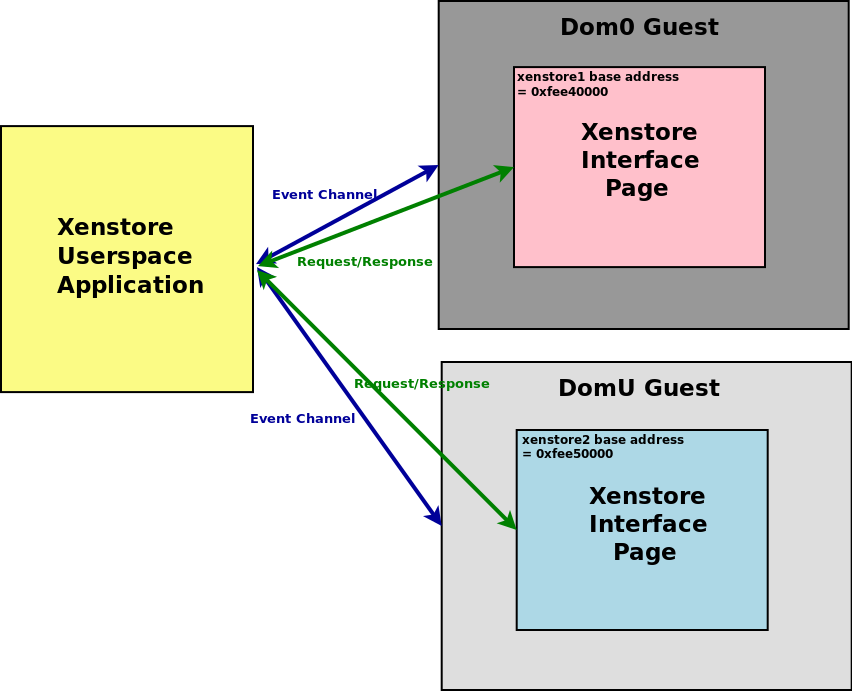
\includegraphics[width=10cm]{xenstore-Page}
	\caption{Communication between Xenstore application and Guests in PHIDIAS}
	\label{xenstore-Page}
\end{figure}

